\section{Introduction}
% par 1: Introduction to the Problem
% Purpose: Define the problem and explain its significance.

%  What is the problem, what is the challenge, and why is it important
% Interfaces are important because they affect data collection. There is no QS interface, and QS is hard, so the problem is how do we design interfaces for QS?

% Version 1
% Designing user interfaces for emerging survey techniques is rare and challenging. Although new techniques offer the potential for more accurate data collection, existing interfaces are often ill-equipped to handle their complexity. We introduce Quadratic Surveys (QS), a surveying technique that applies the principles of Quadratic Voting (QV) to better elicit individual preferences compared to traditional Likert scale surveys~\cite{chengCanShowWhat2021}. Yet, without well-designed interfaces, even the most promising techniques can struggle with user adoption, ultimately threatening survey response quality~\cite{pielotDidYouMisclick2024, kimComparingDataChatbot2019}. The unique challenge of QS lies in its mechanism: respondents allocate a fixed budget of votes, with the cost of casting additional votes on a single option increasing progressively. This cost structure encourages careful trade-offs and promises to improve the accuracy of preference elicitation~\cite{posner2018radical}. At the same time, this mechanism makes responding to QS cognitively challenging. Therefore, this paper seeks to address the key question:~\textit{How can we design interfaces to support participants in completing Quadratic Surveys (QS) more effectively?}

Designing intuitive survey interfaces is crucial for accurately capturing respondents' preferences, which directly impact the quality and reliability of the data collected. Recent Human-Computer Interaction (HCI) studies highlight how certain survey response formats can increase errors~\cite{pielotDidYouMisclick2024, kimComparingDataChatbot2019} and influence survey effectiveness~\cite{ugur2015evaluating}. In this paper, our goal is to introduce an effective interface for~\textbf{Quadratic Surveys (QS)}, a survey tool designed to elicit preferences more accurately than traditional methods~\cite{chengCanShowWhat2021}. Despite the promise of QS, there has been no research on designing interfaces to support its unique quadratic mechanisms~\cite{grovesOptimalAllocationPublic1977}, where participants must rank and rate items --- a task that poses significant cognitive challenges. To popularize QS and ensure high-quality data, this paper addresses the question: \textit{How can we design interfaces to support participants in completing Quadratic Surveys (QS) more effectively?}

\begin{figure}[ht]
    \centering
    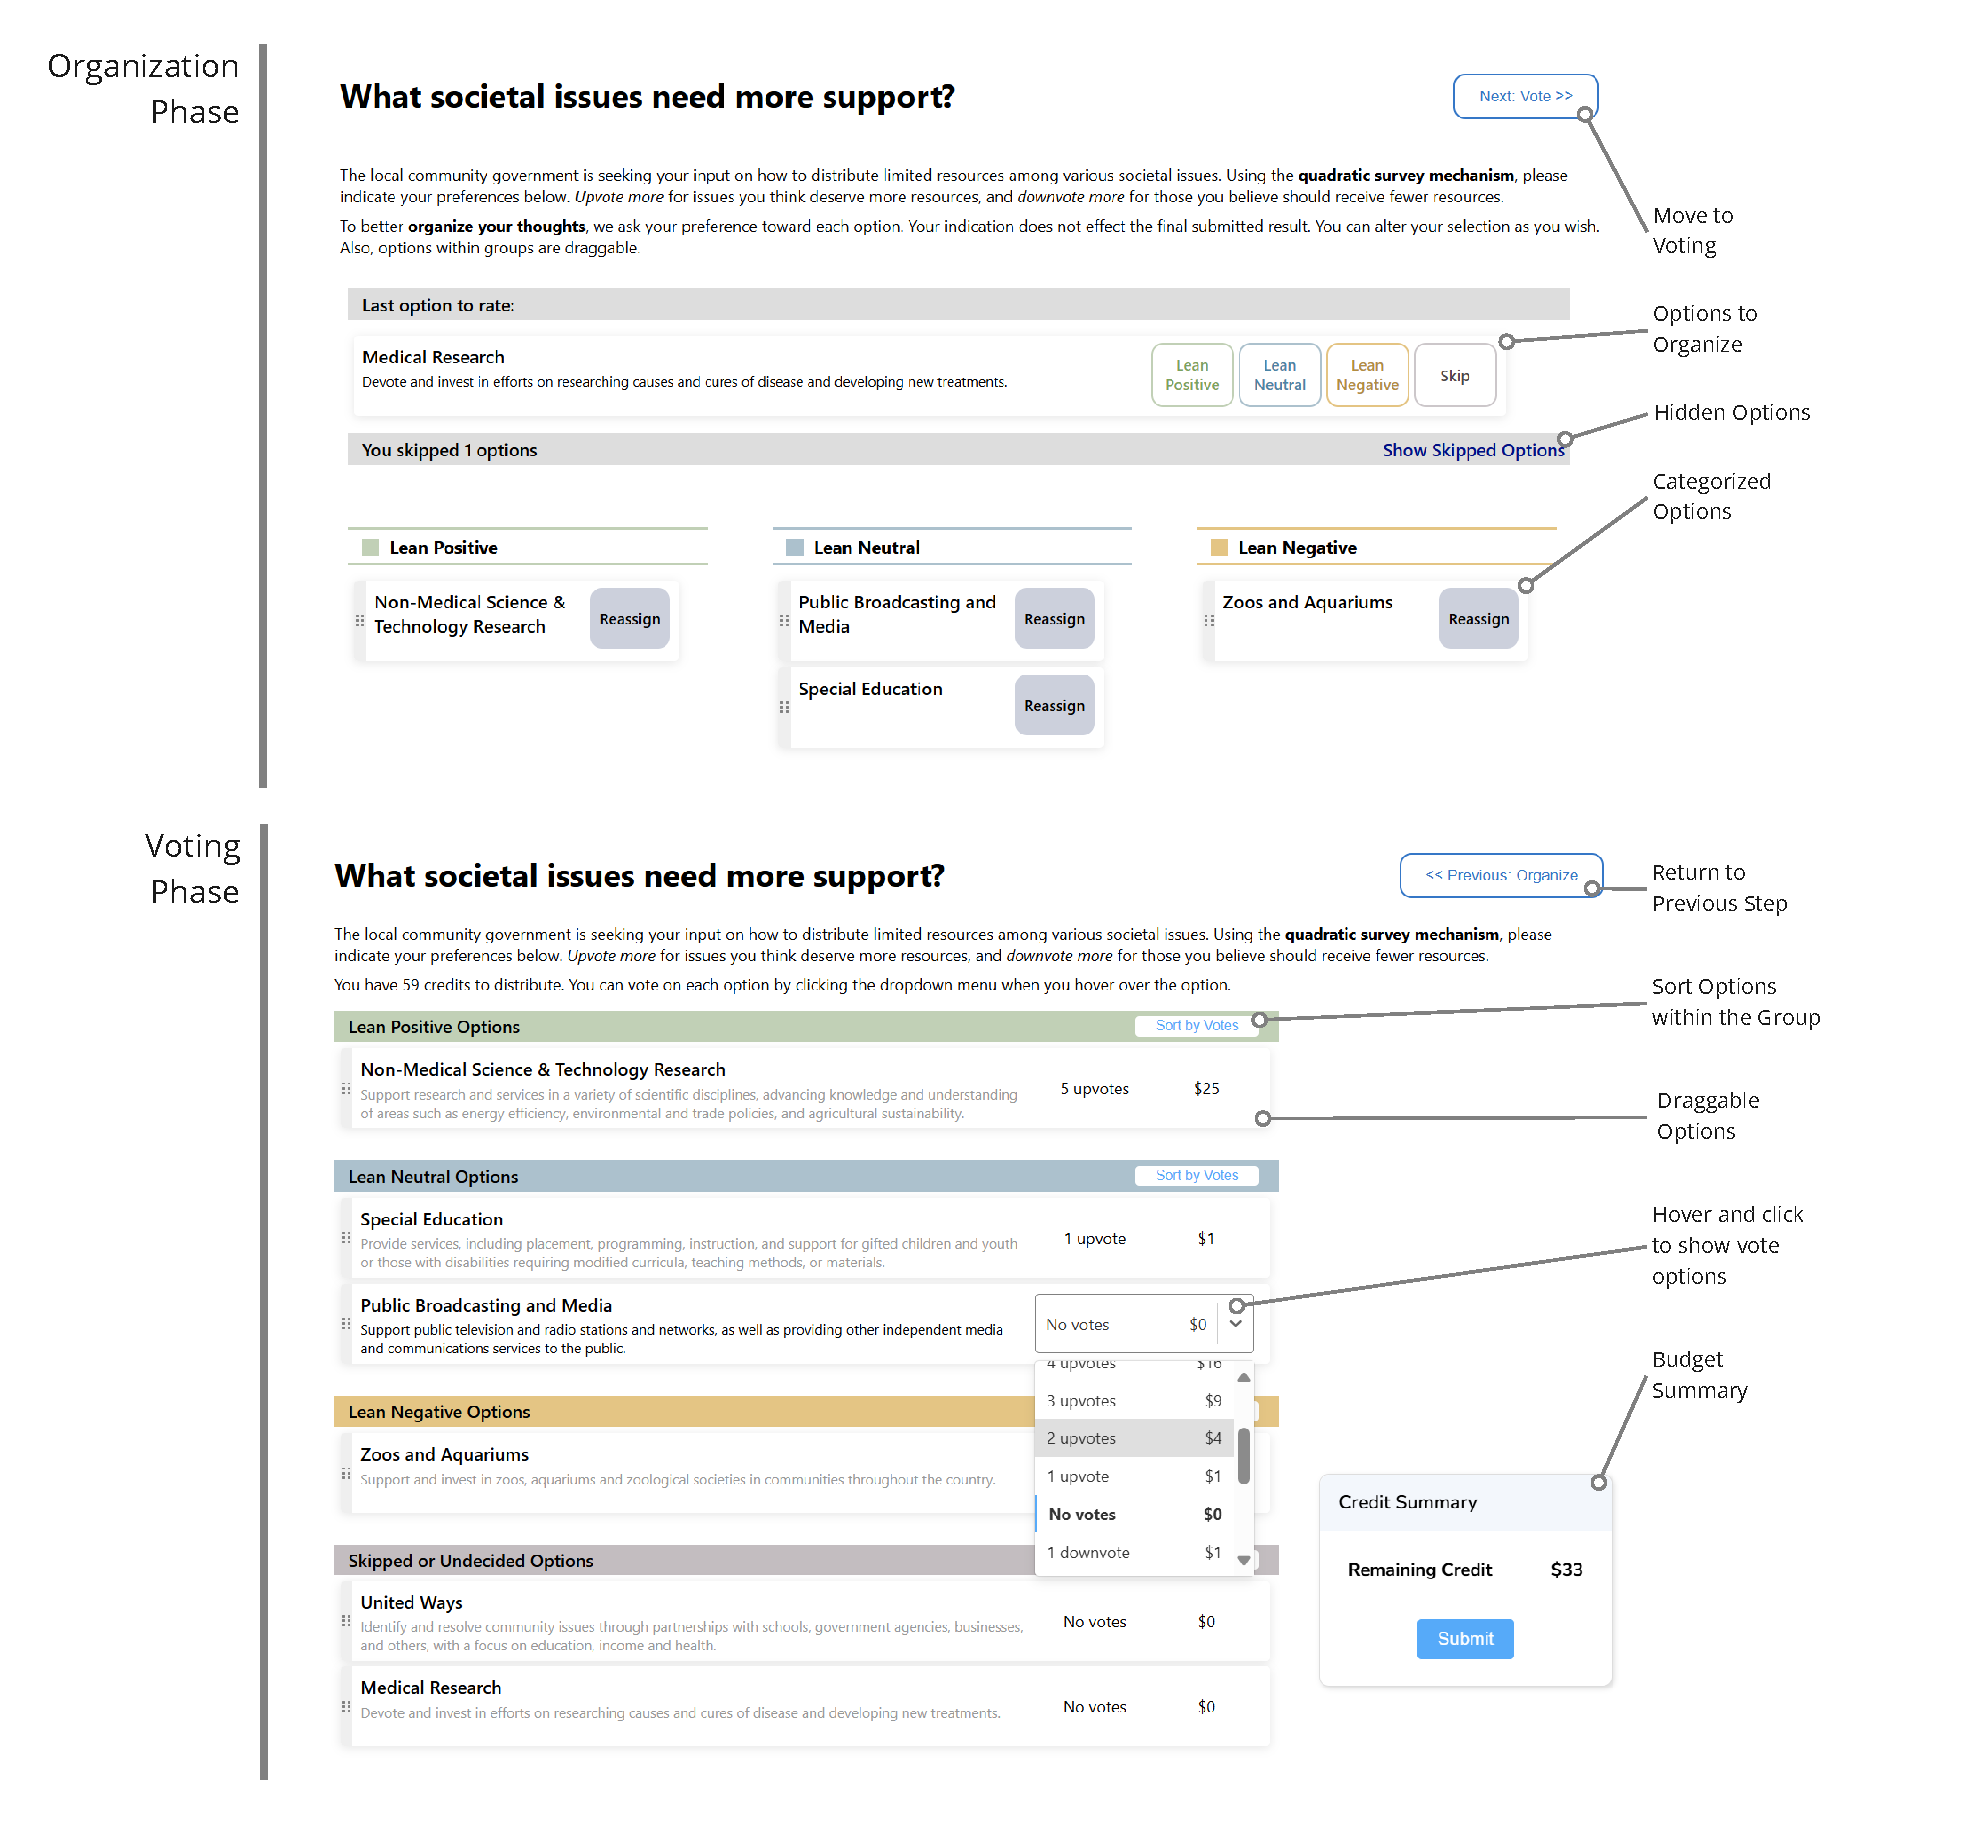
\includegraphics[width=1\textwidth]{content/image/detailed.pdf}
    \caption{The Two-Phase Interface: The interface consists of two phases. Survey respondents can navigate between phases using the top right button. In the organization phase, the interface presented one option at a time to the respondents, and they chose four choices: ``Lean Positive'', ``Lean Neutral'', ``Lean Negative'', or ``Skip''. Skipped options are hidden and can be evaluated later. The chosen options will be listed below. Items can be dragged and dropped across categories or returned to the stack. In the voting phase, options are listed in the order of the four categories. When hovering over each option, respondents can select a vote for that option using the dropdown. Each dropdown contains the cost associated with the vote. A sort button allows ascending sorting within each category. A summary box tracks the remaining credit balance.}
    \label{fig:interactiveInterface}
    \Description{
    This image shows two screen captures: the Organization Phase at the top and the Voting Phase at the bottom. The Organization Phase screen contains a question titled "What societal issues need more support?" with two sections. One section shows a block with descriptions of an option, and to the right of the block are four choices: "Lean Positive," "Lean Neutral," "Lean Negative," or "Skip." The interface also shows a skipped option. Below the block, three columns contain options inside, each showing the option title and a reassign button. In the Voting Phase, the same title and instructions are displayed, but now options are listed by their previously assigned categories (columns). The image shows the mouse hovering over one of the options, revealing a dropdown menu to allocate votes, along with the associated cost in credits. Each category box has a sorting button on the right, allowing users to reorder options within the category. Dots on the left side of the options indicate that drag-and-drop functionality is available for rearranging options. In the lower right corner, a summary box titled "Credit Summary" displays the remaining credit balance for voting. A button in the top left corner allows users to return to the previous Organization Phase.
    }

\end{figure}

% Zoom into two challenges this paper tackles -- zooming in mental demand and cognitive challenges due to the QS mechanism
We envision an effective interface that navigates participants through the complex mechanism and preference construction process\change{, tailored to QS.} QS improves accuracy in individual preference elicitation compared to traditional methods like Likert scales by requiring participants to make trade-offs using a fixed budget of credits, where purchasing $k$ votes for an option in QS costs $k^2$ credits~\cite{quarfoot2017quadratic,chengCanShowWhat2021}. This quadratic cost structure forces respondents to carefully evaluate their preferences, balancing the strength of their support or opposition against the limited budget. \change{As individual preferences are often constructed when given the options, even though this cost structure forces participants to make thoughtful trade-offs, the construction process increases cognitive load, making it mentally taxing to weigh costs, evaluate options, and construct rankings~\cite{lichtensteinConstructionPreference2006}.} Moreover, QS, often referred to as Quadratic Voting (QV) in voting scenarios, can involve hundreds of options~\cite{rogersColoradoTriedNew2019, teamTaiwanDigitalMinister}, increasing the risk of cognitive overload and~\change{taking mental shortcuts~\cite{simonBehavioralModelRational1955, payneAdaptiveStrategySelection1988, tverskyJudgmentsRepresentativeness}}.
% add and possible breakdown interfaces for mental and interfaces to scaffold complex mechanisms

% ================================ %
% par 2: Approaches to Address the Challenges
% Purpose: Describe the existing approaches related to the problem.
% Key Questions:
%  - What are some broad approaches to addressing these challenges? -- there are none.
%  - Do not go into detail about related work but give an idea of the major themes in related work.
%       - No prior research on QS, but there are existing interfaces -> auto calculation as commonality
%       - prior work on interface for reducing cognitive load, preference construction, and voting

To date, existing quadratic mechanism-powered applications simply present options, allow vote adjustments and automatically calculate votes, costs, and budget usage. These designs focused heavily on the mechanics operating the tool, rather than supporting possible challenges these application users faced. Survey interface literature, while addressing decision-making and usability, most focus on traditional surveys that do not share the unique option-to-option trade-offs that QS introduces~\cite{engstrom2020politics, weijtersEffectRatingScale2010, kierujVariationsResponseStyle2010, toepoelSmileysStarsHearts2019, farzandAestheticsEvaluatingResponse2024, pielotDidYouMisclick2024}.~\change{Prior research in HCI and beyond explored techniques to managing cognitive load~\cite{paula2023, oviatt2006human, toepoelSmileysStarsHearts2019, softwareBrad2021, reis2012towards} and scaffolding challenging tasks~\cite{task2014, moderate2021, ibili2019effect, amyChatSensing2018} showing promise in supporting preference construction under QS. Thus, this study aims to bridge this gap.}

% ================================ %
% par 3: Your Proposal
% Purpose: Present your main ideas and proposed solution.
% Key Question:
%  - What are you proposing? Provide a sketch of the major ideas.

\change{We propose a novel interactive two-phase ``organize-then-vote'' QS interface (referred to as the two-phase interface for short, Figure~\ref{fig:interactiveInterface}) after multiple iterations. It aims to facilitate preference construction and reduce cognitive load when making trade-offs through three key elements.} First, the interface scaffolds the preference construction process by having participants initially categorize the survey options into ``Lean Positive,'' ``Lean Neutral,'' or ``Lean Negative.'' This serves as a cognitive warm-up, easing participants into the more complex QS voting task. Second, the interface arranges the options according to these categorizations, providing a structured visual layout. Third, participants can refine the positions of these options using drag-and-drop functionality, giving them greater control and agency in the preference-construction process. %These design features are aligned with preference construction theory and build upon prior research in interface design to reduce cognitive load and enhance user engagement.

To explore how these interface elements mitigate the cognitive load and support preference construction in Quadratic Surveys, we pose the following research questions:
\begin{itemize}
    \item RQ1. How does the number of options in Quadratic Surveys impact respondents' cognitive load?
    \item RQ2a. How does the two-phase interface impact respondents' cognitive load compared to a single-phase text interface?
    \item RQ2b. What are the similarities and differences in sources of cognitive load across the two interfaces?
    \item RQ3. What are the differences in Quadratic Survey respondents' behaviors when coping with long lists of options across the two-phase interface and the single-phase text interface?
\end{itemize}

% ================================ %
% par 4: Main Findings
% Purpose: Summarize the key findings from your work.
% Key Question:
%  - What are the main findings?
We invited 41 participants to a lab study comparing our two-phase interface with a baseline to understand how different interface designs and option lengths ($6$ options or $24$ options) impact cognitive load. 


\change{Self-reported cognitive load using the NASA Task Load Index~(NASA-TLX) and semi-structured interviews identified common challenges in Quadratic Surveys (QS), such as preference construction and budget management, while highlighting differences between text and two-phase interfaces. The two-phase interface fostered more strategic engagement with survey options considering broader impacts in the long QS, reduced time pressure in the short QS, and participants expressed greater affirmative satisfaction (e.g., 'feeling good'). Quantitative results showed that the organizing phase in the two-phase interface led participants, particularly in long surveys, to traverse the option list less often without reducing edits and spend more time per option, signifying deeper engagement and a shift toward more strategic thinking when constructing their preferences.}

% Qualitative findings, measured using the NASA Task Load Index~(NASA-TLX) and semi-structured interviews, revealed that participants using the two-phase interface experienced cognitive demand more from strategic, holistic thinking compared to personal relevance and operational tasks, particularly in longer surveys. Quantitative results showed that, although participants spent more time per option, they made faster decisions during the voting phase, suggesting a more efficient distribution of cognitive effort. We concluded that the two-phase interface mitigated cognitive overload in long QS surveys and shifted mental load toward more strategic thinking, reducing reliance on mental shortcuts like satisficing~\cite{simonBehavioralModelRational1955}.

% ================================ %
% par 5: Main Contributions
% Purpose: Identify and explain the primary contributions of your work.
% Key Structure:
%  1. Line 1: Identify your contribution—conceptualization, framework, interface, algorithm, etc.
%  2. Line 2: Contrast your contribution with prior work.
%  3. Line 3: Explain how you accomplished your contribution.
%  4. Line 4: Emphasize the impact of the contribution—why should anyone care?

\paragraph{Contributions}
We contribute to the HCI community by proposing the first interface specifically designed for QS and QV-like applications, aimed at reducing cognitive challenges and scaffolding preference construction through a two-phase interface with direct manipulation. Before our work, no research had explored QS interfaces, particularly for long QS prone to cognitive overload. Few studies in HCI address interfaces for surveys and questionnaires.~\change{Our study demonstrated how user interfaces can facilitate preference construction in situ and promote deeper engagement with survey options through interface elements. Additionally, this paper offers the first in-depth qualitative analysis of user experiences among Quadratic Mechanism applications, identifying usability challenges and key factors contributing to cognitive load.} The impact of our contribution extends beyond QS, offering design implications for other preference-elicitation tools in~\change{multi-option scenarios}. By making QS easier to use and more accurate, our design also encourages wider adoption among researchers and practitioners.~\change{Finally, our work lays the groundwork for future quadratic mechanisms interface design to better facilitate individuals in communicating their preferences.}

% ================================ %
% Removed text
% Surveys are a ubiquitous tool for collective decision-making, providing decision-makers with aggregated opinions that directly shape the outcomes for those surveyed. For example, states utilize referendums to form policy decisions, organizations like the Pew Research Center survey public perspectives on societal challenges in the United States, and city councils hold forums to gather community concerns.
% and private sectors~\cite{Gov4gitDecentralizedPlatform2023}.
% xiaoTellMeYourself2020, 

% ================================ %